\chapter{Разработка экспериментального стенда}
\label{cha:chap5}

\section{Выбор компонентов и устройств для реализации узлов системы}
\label{sec:choose}

В данном разделе будут определены элементы и устройства для реализации узлов, определённых в \ref{sec:nodes}.

В качестве мозга для реализации алгоритма управления был выбран микроконтроллер STM32F411RET (Рисунок \ref{pic:mc}), который содержит всю необходимую периферию  (поддерживает генерацию ШИМ, имеет аналого-цифровой преобразователь (АЦП), таймеры и имеет возможность передачи информации по последовательный протоколу связи).

\begin{figure}[!h]
\centering
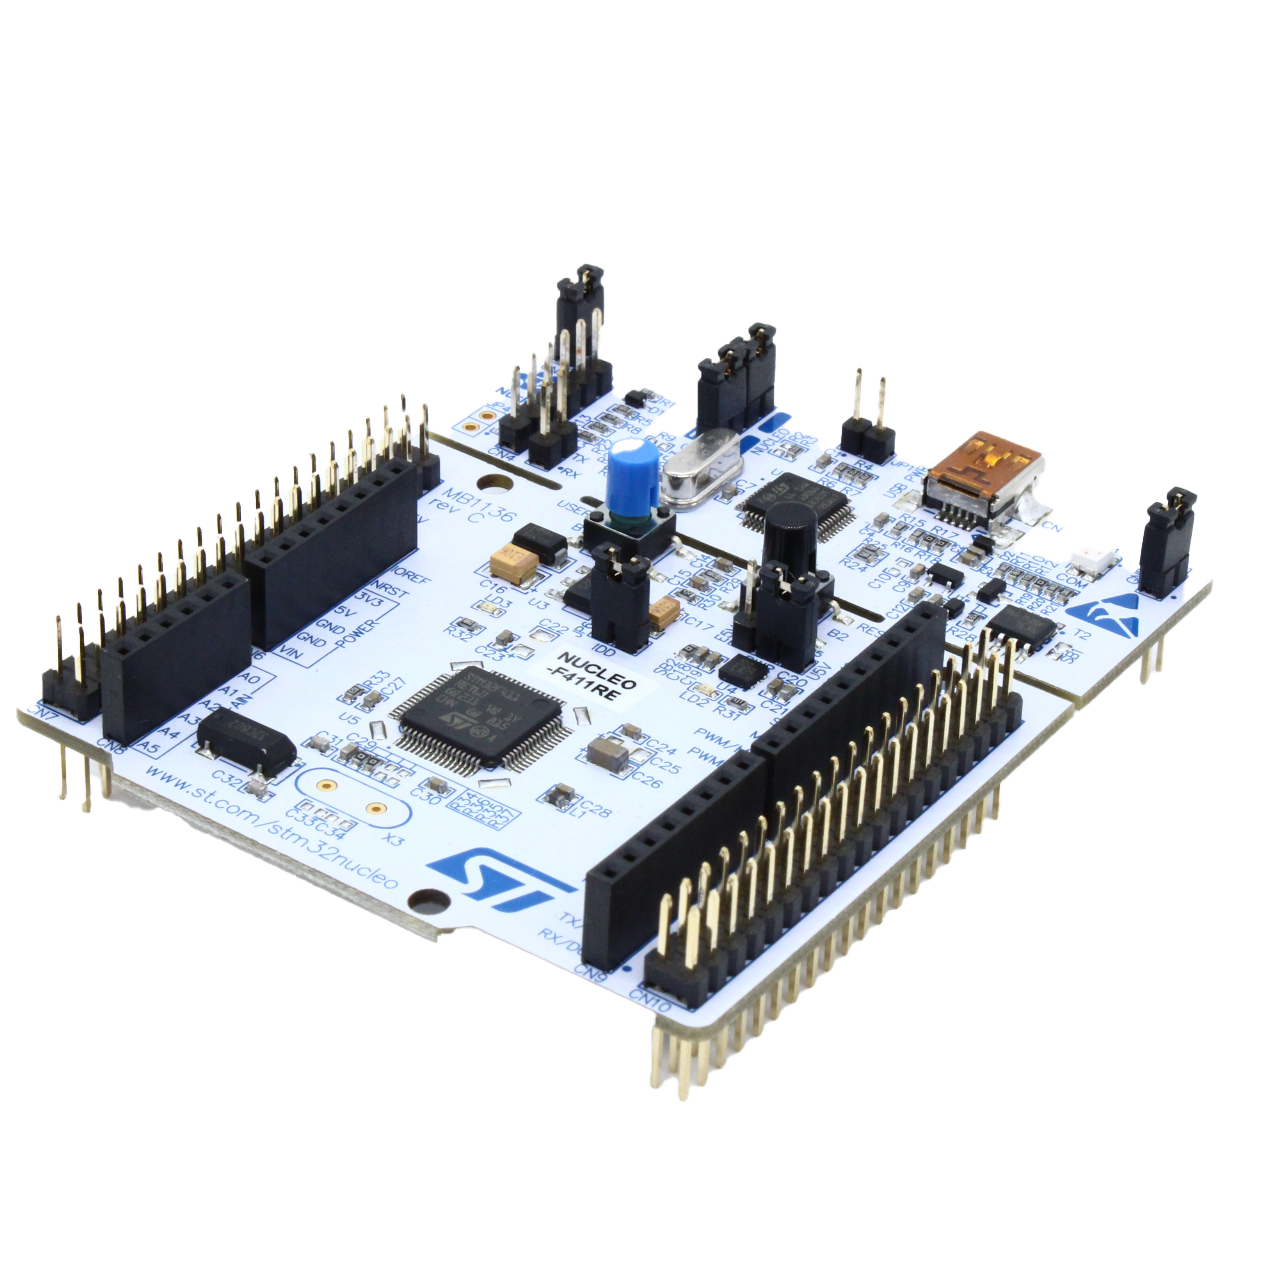
\includegraphics[width=0.7\textwidth]{inc/img/mc.png}
\caption{Микроконтроллер STM32F411RET на базе Nucleo64}
\label{pic:mc}
\end{figure}

Инвертор, датчики для определения напряжения и тока фаз реализованы на отдельной печатной плате, рассмотренной в \ref{sec:driver}. 

За объект управления взят двигатель Racerstar BR2208 1100KV (Рисунок \ref{pic:motor}), параметры которого были перечислены при моделировании в \ref{sec:model_res}.

\begin{figure}[!h]
\centering
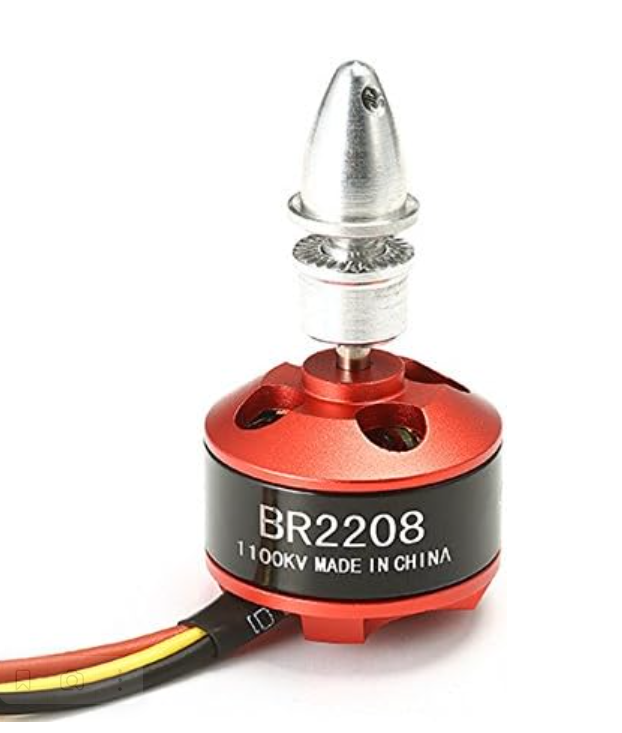
\includegraphics[width=0.5\textwidth]{inc/img/motor.png}
\caption{БДПТ Racestar BR2208 1100KV}
\label{pic:motor}
\end{figure}

Для питания двигателя был выбран блок питания на 12 В/5 А (Рисунок \ref{pic:power}), которого будет достаточно для питания двигателя в условиях работы без нагрузки или в условиях малых нагрузок и который обеспечит сохранность всей электрической схемы в случае короткого замыкания.

\begin{figure}[!h]
\centering
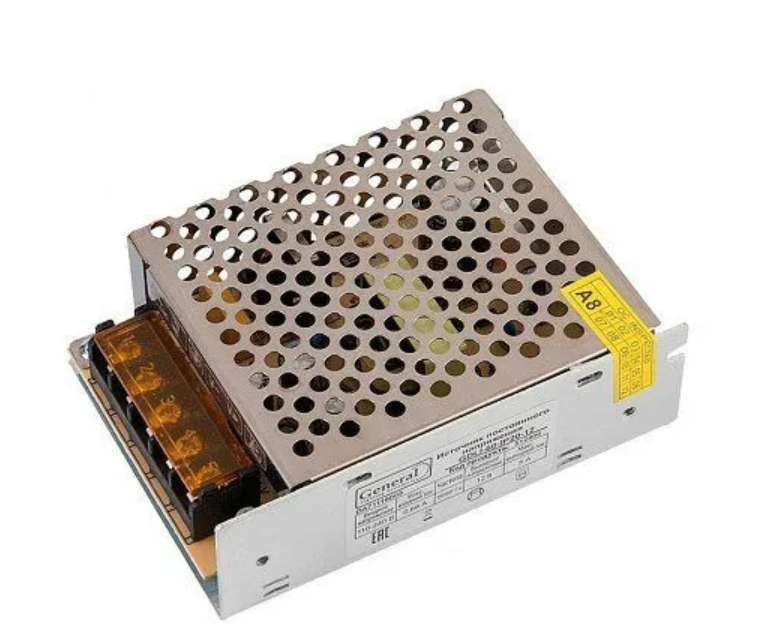
\includegraphics[width=0.7\textwidth]{inc/img/power.png}
\caption{Блок питания двигателя}
\label{pic:power}
\end{figure}
\clearpage
\section{Реализация драйвера двигателя}
\label{sec:driver}

Для реализации силовой части был спроектирован собственный драйвер БДПТ в среде проектирования Altium Designer.

\subsection{Инвертор}

Для 3-фазного инвертора были использованы полумостовые драйверы IR2104STRPBF для каждой фазы, которые служат для преобразования напряжений микроконтроллера в напряжения, достаточные для открытия ключей, в качестве которых выступают mosfet транзисторы IRLR2705PBF. Также драйверы выбранные драйверы транзисторов исключают возможность одновременного открытия верхнего и нижнего ключей, исключая возникновение короткого замыкания в этом случае.

Они имеют два входа для регулирования ($IN$ и $\overline{SD}$) и два выхода к транзисторам ($HO$ и $LO$). Зависимость сигналов выхода от значений входа изображена на Рисунке \ref{pic:driver_sw}. В нашем случае нижний вход будет служить для подачи на него ШИМ сигнала, а с помощью верхнего будет регулироваться, какой выход и, соответственно, какой транзистор открыть (при $IN=1$ открывается верхний ключ, при $IN=0$ открывается нижний ключ).

\begin{figure}[!h]
\centering
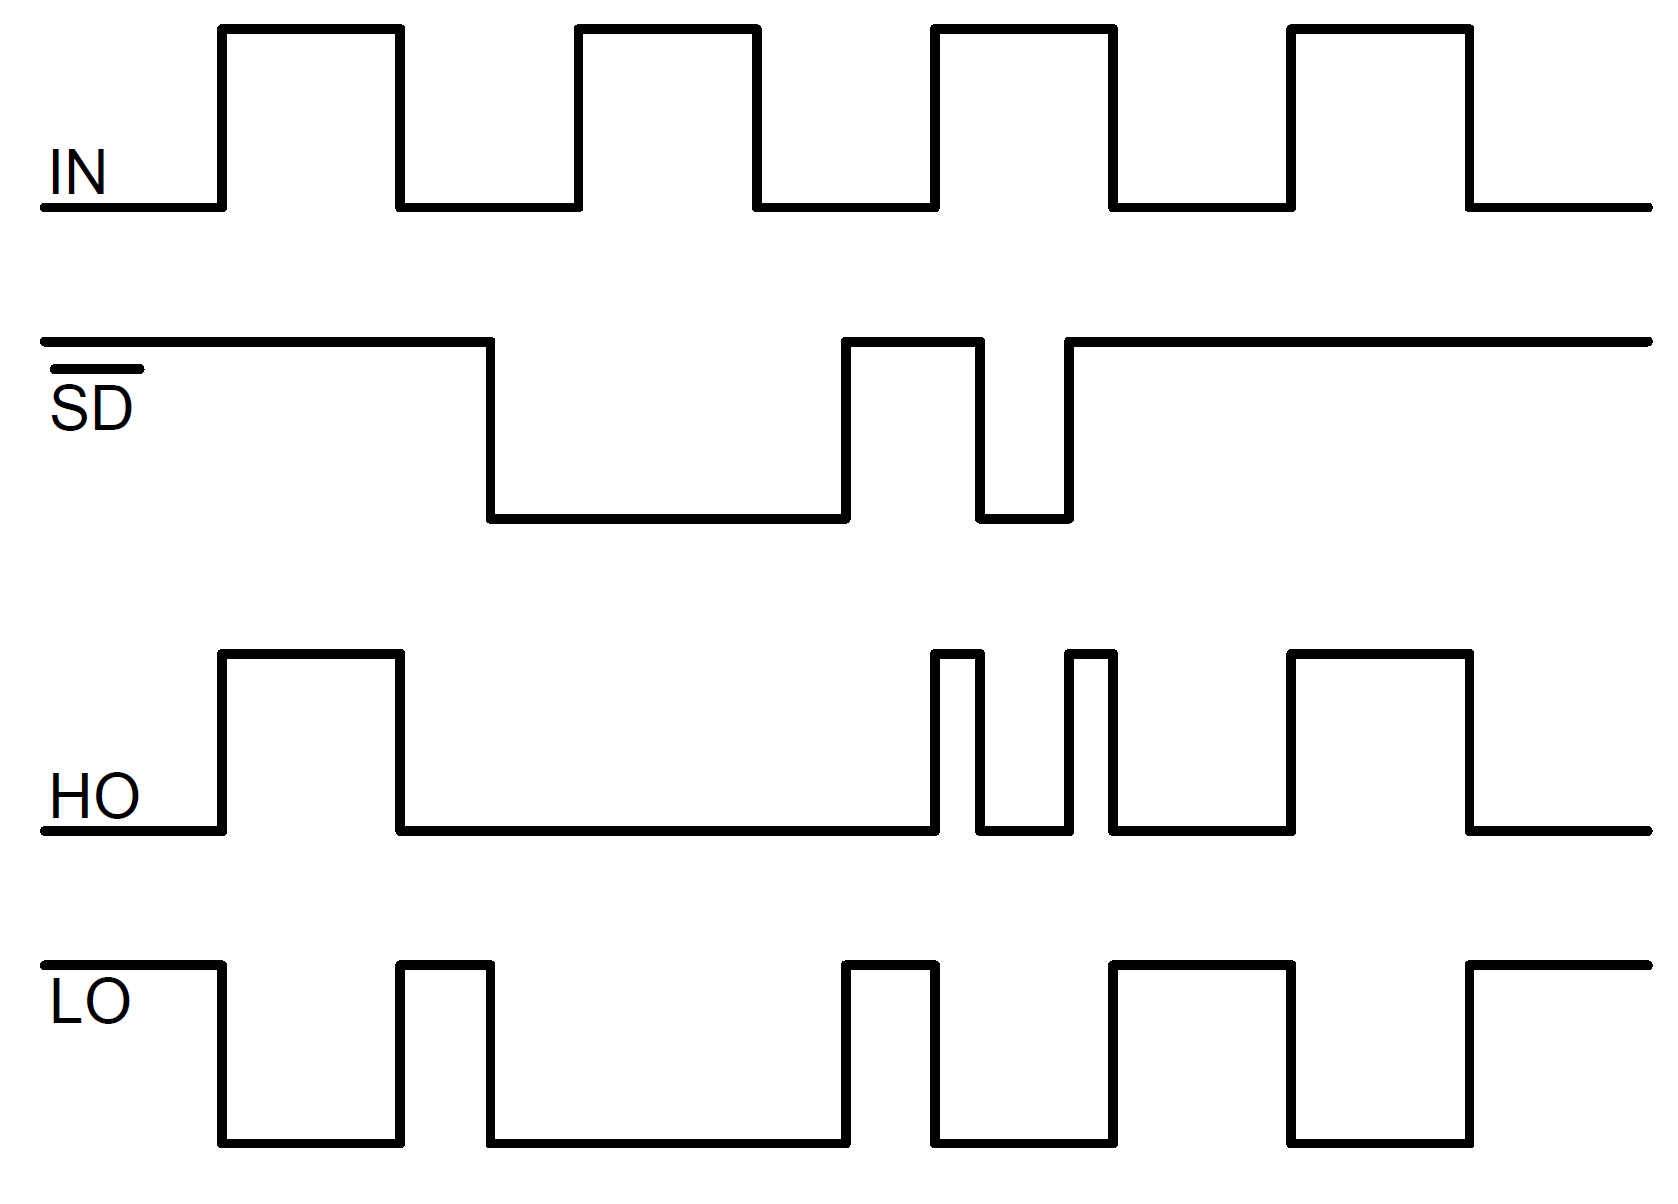
\includegraphics[width=0.7\textwidth]{inc/img/driver_sw.png}
\caption{Зависимость значений входов/выходов для IR2104STRPBF}
\label{pic:driver_sw}
\end{figure}

Также параллельно фазам двигателя установлены диоды, которые препятствуют протеканию обратного тока катушек, которыми являются фазы двигателя, во время смены состояния ключей.

Общая схема силовой части изображена на Рисунке \ref{pic:dr_power}.

\begin{figure}[!h]
\centering
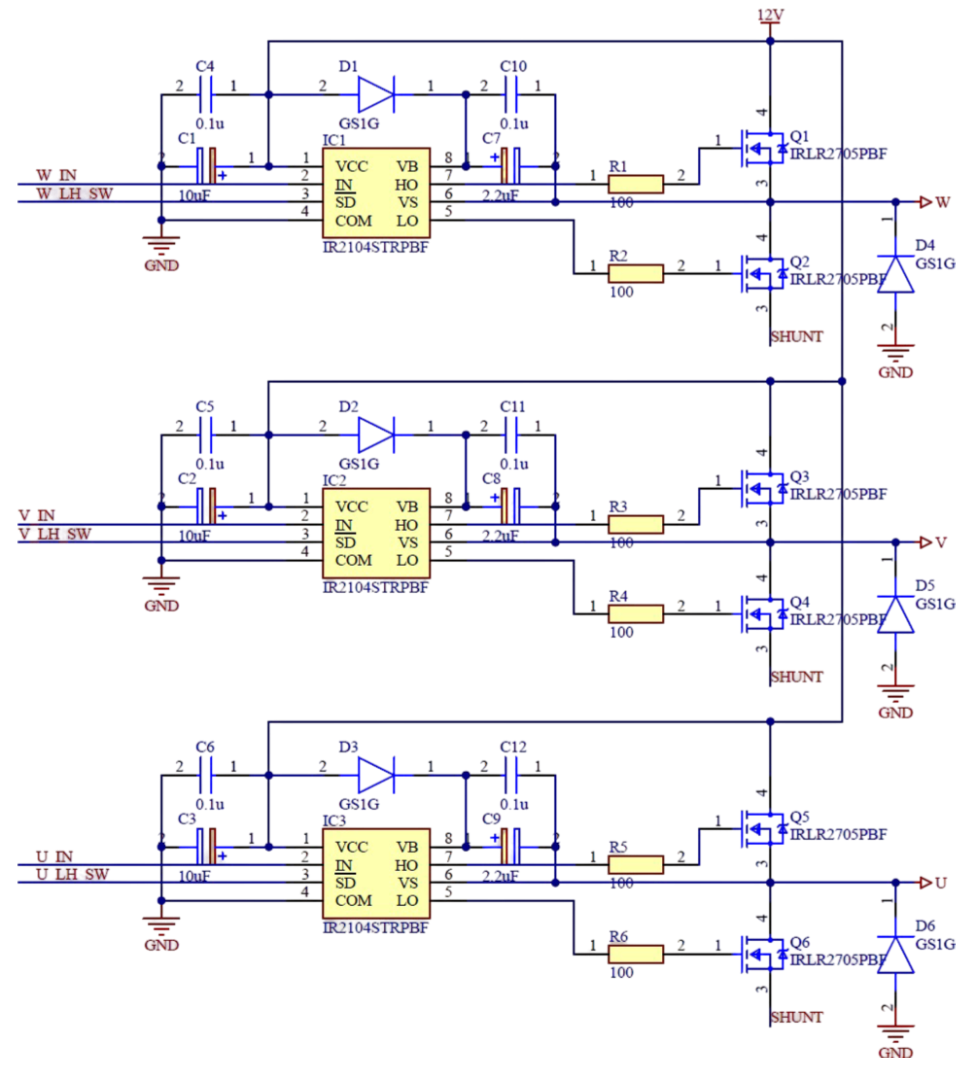
\includegraphics[width=\textwidth]{inc/img/dr_power.png}
\caption{Схема силовой части ($W$, $V$, $U$ --- фазы двигателя, $SHUNT$ --- сигнал, уходящий к датчику тока, $12V$ --- питание $12$ В, $WVU_{IN}$, $WVU_{LH_SW}$ --- входы для управления ключами драйвера)}
\label{pic:dr_power}
\end{figure}
\clearpage
\subsection{Измерительная часть}

Для измерения тока используется датчик тока на основе ACS712ELCTR-05B-T, позволяющий преобразовать ток, текущий через него в напряжение в диапазоне от $0$ до $5$ В. Схема измерения тока изображена на Рисунке \ref{pic:cur_sens}.

\begin{figure}[!h]
\centering
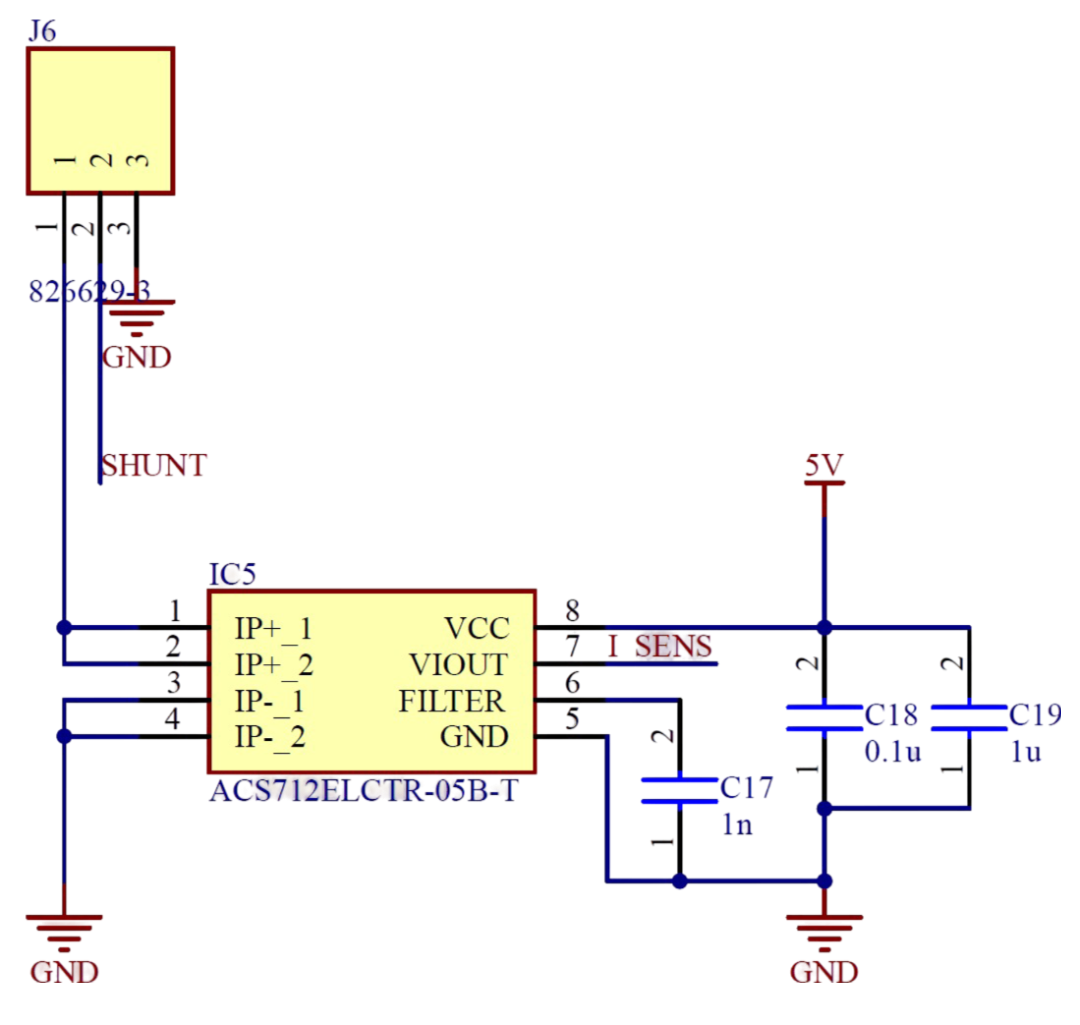
\includegraphics[width=0.5\textwidth]{inc/img/cur_sens.png}
\caption{Схема с датчиком тока ($SHUNT$ --- сигнал с фаз двигателя, $5V$ --- питание $5$ В, $I_{SENS}$ --- сигнал выхода датчика тока)}
\label{pic:cur_sens}
\end{figure}

Для измерения напряжения на фазах необходимо использовать делители напряжения для преобразования из диапазона $0-12$ В в диапазон $0-5$ В. Также устанавливается конденсатор для избавления от высокочастотных шумов. Схема изображена на Рисунке 

\begin{figure}[!h]
\centering
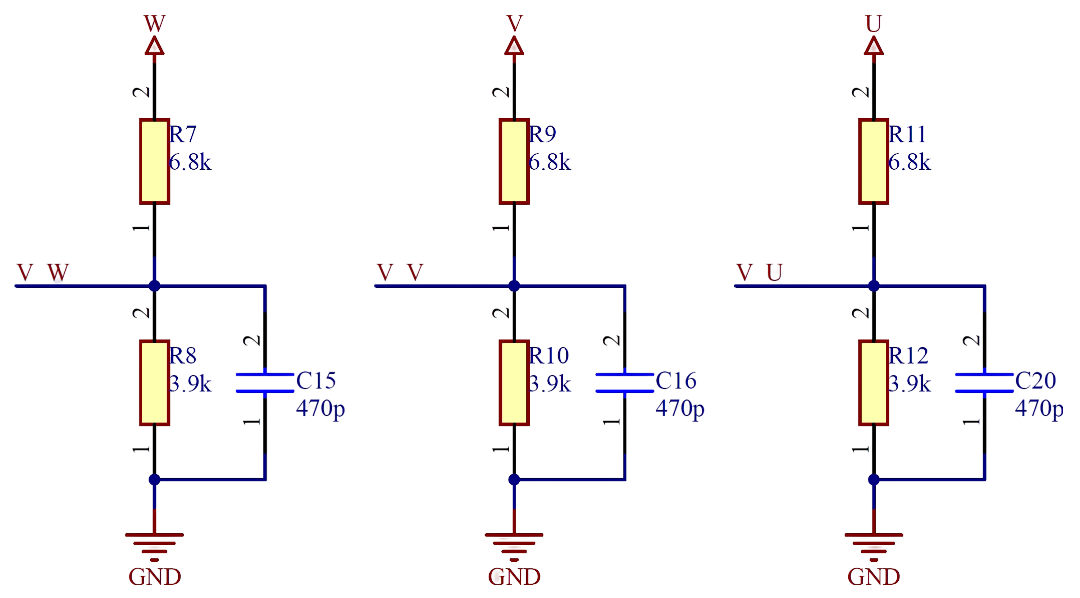
\includegraphics[width=0.7\textwidth]{inc/img/dr_dels.png}
\caption{Схема с делителями напряжения ($WVU$ --- фазы двигателя, $V_{VWU}$ --- сигналы с напряжениями фаз))}
\label{pic:dr_dels}
\end{figure}

\subsection{Подключение входов и выходов платы}

Питание платы осуществляется двумя уровнями напряжений --- $12$ и $5$ В. Первое идёт на питание двигателя и формируется блоком питания, второе служит для питания датчика тока и идёт от микроконтроллера. От микроконтроллера также идут сигналы для управления драйверами транзисторов.

От плату на входы АЦП микроконтроллера идут сигналы с датчика тока и делителей напряжения. Однако на плате напряжения выходных сигналов приведены в диапазоне $0-5$ В, а АЦП выбранного микроконтроллера работает с напряжениями $0-3,3$ В, поэтому не можем напрямую подключить сигналы с платы и необходимо использовать преобразователь логических уровней. Был выбран преобразователь на основе TXS108E.

\begin{figure}[!h]
\centering
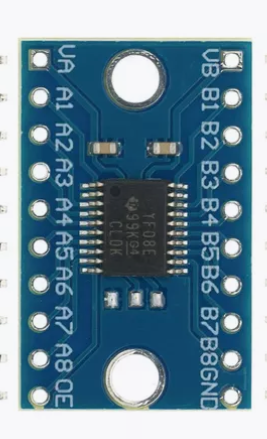
\includegraphics[width=0.3\textwidth]{inc/img/log_transf.png}
\caption{Преобразователь логических уровней на базе TXS108E}
\label{pic:log_transf}
\end{figure}

Подключение фаз двигателя осуществляется через 2-х контактный клеммник, как и напряжения питания $12$ В. Остальные сигналы подключаются посредством штырьевых разъёмов.

\subsection{Общий вид платы}

На Рисунке \ref{pic:dr_view1} приведён вид платы, сгенерированный в редакторе, а на Рисунке \ref{pic:dr_view2} изображена уже изготовленная и распаянная плата.

\begin{figure}[!h]
\centering
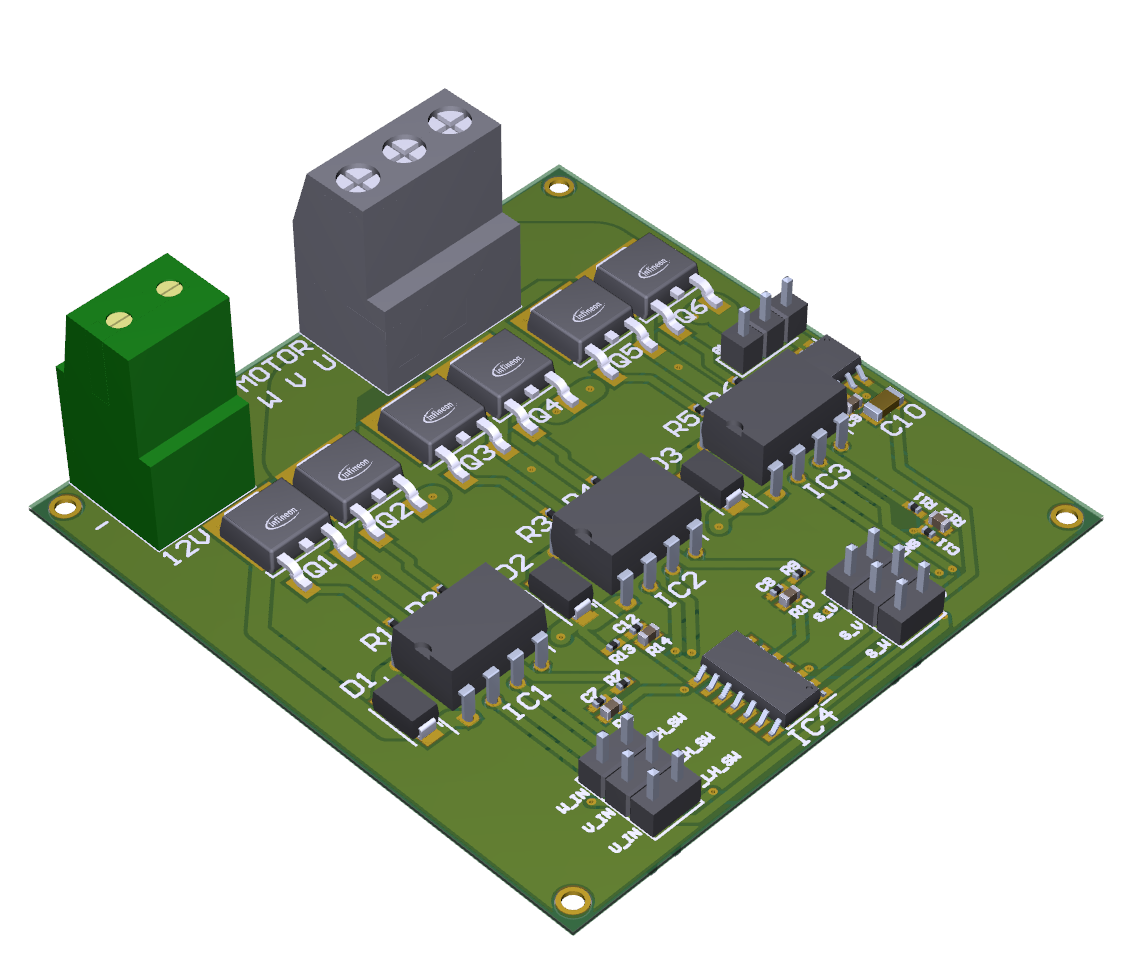
\includegraphics[width=0.7\textwidth]{inc/img/dr_view1.png}
\caption{Вид платы из Altium Designer}
\label{pic:dr_view1}
\end{figure}

\begin{figure}[!h]
\centering
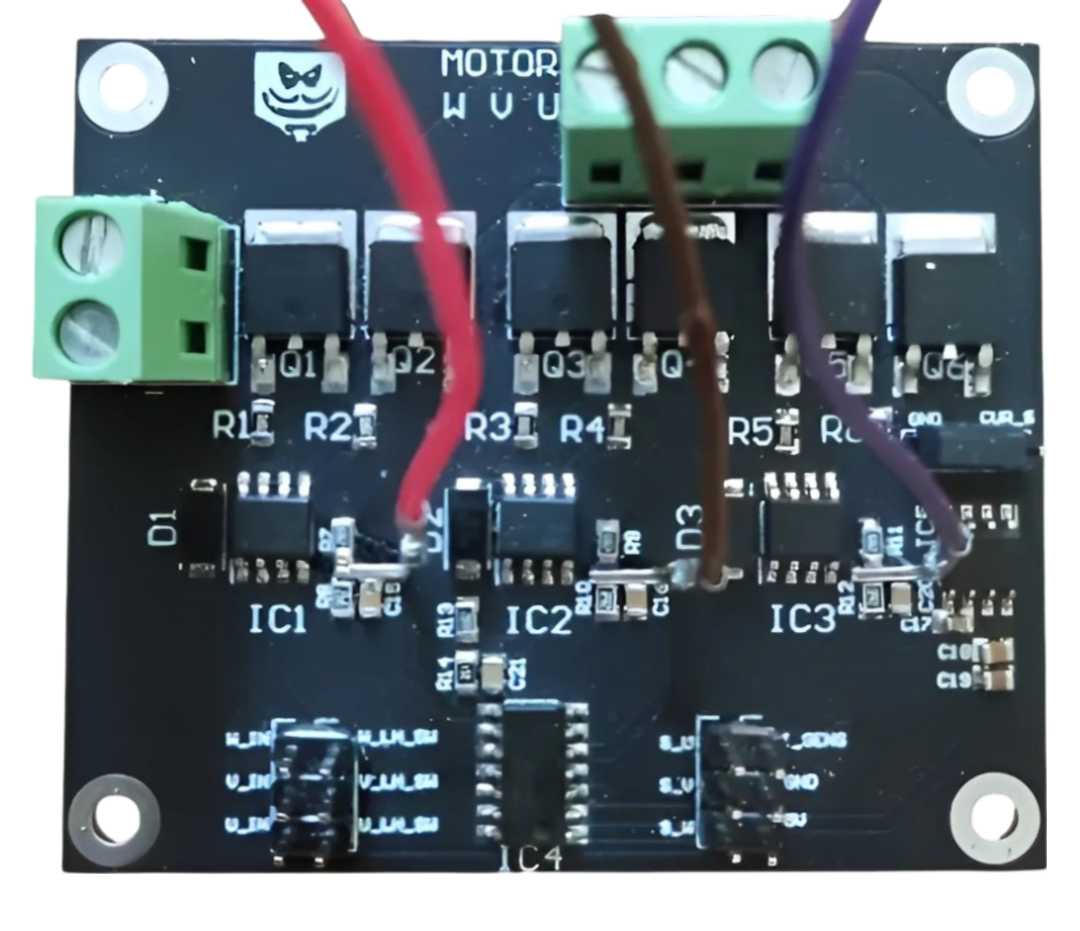
\includegraphics[width=0.7\textwidth]{inc/img/dr_view2.png}
\caption{Вид изготовленной платы}
\label{pic:dr_view2}
\end{figure}
\clearpage
\section{Вид стенда}

На основе выбранных компонентов и узлов был собран стенд для экспериментальных исследований, представленный на Рисунке \ref{pic:stand}.

\begin{figure}[!h]
\centering
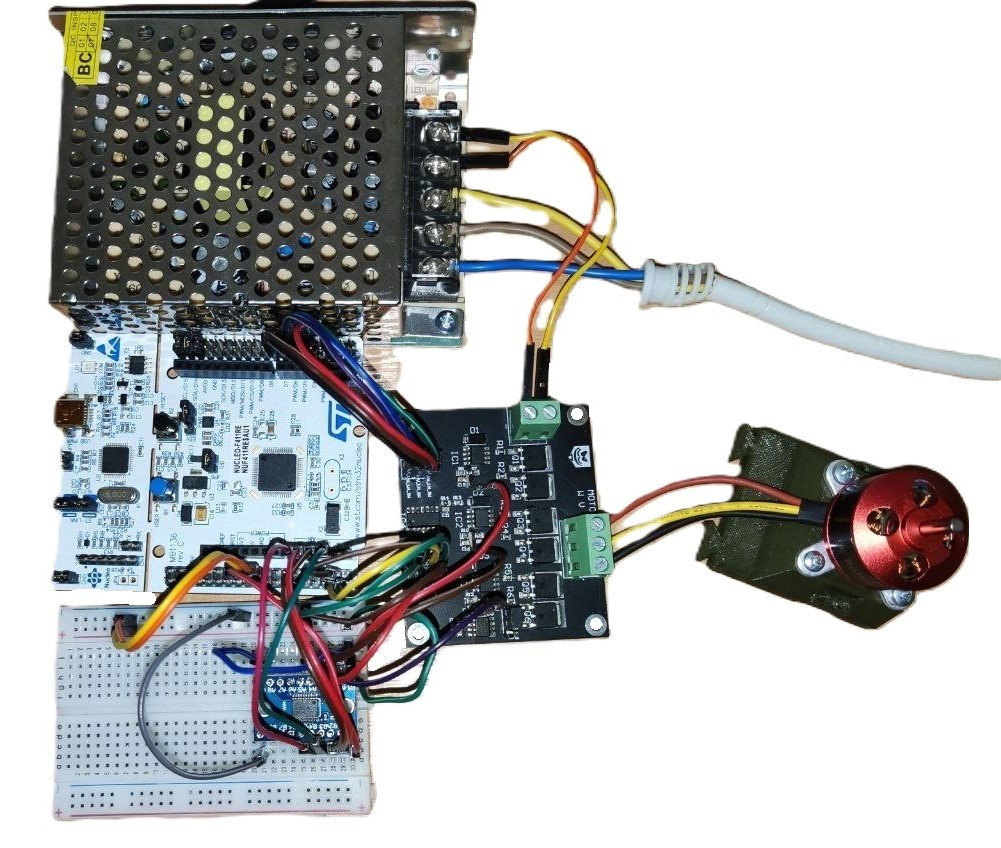
\includegraphics[width=0.7\textwidth]{inc/img/stand}
\caption{Экспериментальный стенд}
\label{pic:stand}
\end{figure}